\documentclass{sig-alternate}
\usepackage[utf8]{inputenc}
\usepackage{graphics}
\usepackage{hyperref}


\begin{document}
%opening
%
% --- Author Metadata here ---
\conferenceinfo{WOODSTOCK}{'97 El Paso, Texas USA}
%\CopyrightYear{2007} % Allows default copyright year (20XX) to be over-ridden - IF NEED BE.
%\crdata{0-12345-67-8/90/01}  % Allows default copyright data (0-89791-88-6/97/05) to be over-ridden - IF NEED BE.
% --- End of Author Metadata ---

\title{Assessment, design and implementation of a private cloud for MapReduce applications}

\numberofauthors{4}

\author{
%
\alignauthor
Patricia Gonz\'alez G\'omez\\
       \affaddr{Department of Electronics and Systems at UDC}\\
       \affaddr{Campus de Elvi\~na s/n, 15007}\\
       \affaddr{A Coru\~na, Spain}\\
       \email{patricia.gonzalez@udc.es}
% 2nd. author
\alignauthor
Jos\'e Carlos Cabaleiro Dom\'inguez\\
       \affaddr{Institute for Clarity in Documentation}\\
       \affaddr{P.O. Box 1212}\\
       \affaddr{Dublin, Ohio 43017-6221}\\
       \email{jc.cabaleiro@usc.es}
% 3rd. author
\alignauthor
Tom\'as Fern\'andez Pena\\
       \affaddr{The Th{\o}rv{\"a}ld Group}\\
       \affaddr{1 Th{\o}rv{\"a}ld Circle}\\
       \affaddr{Hekla, Iceland}\\
       \email{tf.pena@usc.es}
\and  % use '\and' if you need 'another row' of author names
% 4th. author
\alignauthor
Marcos Salgueiro Balsa\\
       \affaddr{Brookhaven Laboratories}\\
       \affaddr{Brookhaven National Lab}\\
       \affaddr{P.O. Box 5000}\\
       \email{marcos.salgueiro@gmail.com}
}

\maketitle



\begin{abstract}
The extraordinarily vast amount of information generated as a byproduct of Internet usage, has been embodying an increasing burden to traditional procedures and models, unable to handle it efficiently due to its heterogeneous nature. Besides, as the volume of information grows so does the size of the datacenter required to process and store it, quickly overloading its full capacity when demand peaks. Together ---\emph{not relational} data and uneven demand distribution--- they shape the basis of modern data-driven request servicing.

A series of technologies have been developing lately to manage this scenario. Two of the most highlighted among them are \emph{MapReduce} and \emph{Cloud Computing}. \emph{MapReduce} was introduced in \cite{Dean:2004:MSD:1251254.1251264} to abstract the common difficulties linked to distributed processing on large clusters. \emph{Cloud Computing}, on the other hand, agglutinates miscellaneous subsystems forming a unified interface to flexibly deploy and manage virtual clusters.

This paper explores their potential symbiosis, in order to create a robust and scalable environment, to execute \emph{MapReduce} workflows regardless of the underlaying infrastructure. It also details a proof of concept implementation using open source tools, similar to Amazon's own \emph{Elastic MapReduce}.
\end{abstract}



\keywords{Distributed Processing, Virtualization, Cloud Computing, MapReduce, OpenStack, Hadoop.\\}



\section{Introduction}\label{sec:int}
\noindent The proliferation of Internet-enabled handhelds and the continuously improving access speed, have set a background in which user services are becoming heftier ---from SQ Video yesterday to HD today and 4K tomorrow---, are being consumed throughout the day and are requiring an increasing amount of user-related data ---GPS position, locale, personal settings, filters, previous searches or purchases, connections, friends, retweets, etc.--- to take into account. It is this last trait what have been representing the biggest trouble: the \emph{class} of data packed within these services cannot be modeled by traditional standards, as it lacks a relational structure.

While some argue that every miniworld may be \emph{transformed} into a Relational Model, it is the necessity to lay out the data structure before information can be saved and put to use what poses a central obstacle in making these models adapt to such a swiftly mutating data. As figure \ref{fig:trend} depicts, the gap between relational and unstructured information continues to widen, that is why there has been an explicit push off schema-driven modeling towards loosely-structured representations.

\begin{figure}[tbp]
\centering
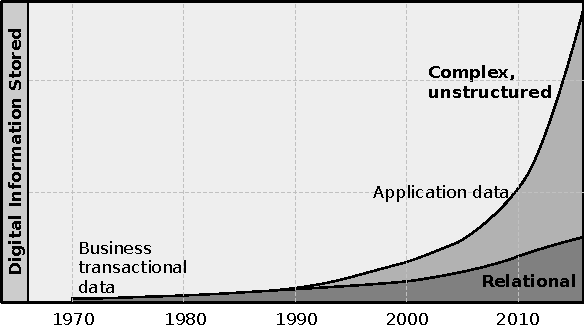
\includegraphics[width=0.45\textwidth]{img/001}
\caption{Unstructured and relational data volume evolution. Source: \emph{Cloudera Inc.}}
\label{fig:trend}
\end{figure}

So, relaying on \emph{schemaless} data definition allows to better cope with unstructured information. There are still, however, two dimensions to discuss: data volume and non-uniform access distribution.

To handle data flowing in at Internet scale there has to be devised a distributed processing model beyond large clusters, high capacity networks and intelligent load balancers. To deal with that sea of data, \emph{MapReduce} processing model splits input all the way down to unrelated pairs of \emph{unique} key and key-related data. Using the approach to uniquely identify each \emph{atomic} piece of information, allows to easily apply a fair distribution policy across participating nodes able to reduce network transfers and to recover from failure.

Finally, clusters' capacity has to be able to accommodate a variable number of information requests per second, reducing idle node time without implying a loss in service quality. An ideally suited technique to that end is \emph{Cloud Computing}. \emph{Cloud Computing} has been making headlines as of late praised for its inherent nature to scale-out virtual deployments effortlessly, and so, capable of stretching and shrinking computational power with demand needs.

Inasmuch as \emph{MapReduce} and \emph{Cloud Computing} together may prove useful in servicing a potential world of data consumers, it is easy to understand the growing interest in both technologies. Currently, the best known example of a unified approach to said technologies is \emph{Amazon Elastic MapReduce} (EMR) \cite{emr:2013:online}. Nonetheless, there are other implementations focusing on extending EMR's functionality, either by surpassing its constraints ---information must be made semi-public and \emph{MapReduce} workflows need to be executed on Amazon's installation--- with \emph{Resilin} \cite{resilin}, \emph{Savanna} \cite{savanna:2013:online} or \emph{Dynamic MapReduce} \cite{dynamicmapreduce}, or by reusing its cloud interface to build a \emph{MapReduce} platform upon like with \emph{Cloud MapReduce} \cite{cloudmapreduce}.

The major contribution of this work is a simple and unified interface to manage \emph{MapReduce} computations, leveraging any existing \emph{IaaS} deployment with a little customization, while providing an automatic one node test installation based on \emph{OpenStack} and \emph{Apache Hadoop}. We have called our implementation \emph{qosh} and it has been written in \emph{Python}.

Section \ref{sec:arch} details \emph{qosh}'s architecture and self-installing deployment structure. Section \ref{sec:hadvm} describes how the \emph{Apache Hadoop} virtual machine was built up. Section \ref{sec:execution} goes through a complete execution cycle, identifying key points of the process. Section \ref{sec:performance} reviews qosh performance when deployed on a real cluster. ----------------------------------------------



\section{Architecture}\label{sec:arch}
\noindent \emph{qosh}'s setup defaults to a single node installation in which both infrastructure and execution environment are configured. Figure \ref{fig:arch1} precisely depicts the layered configuration. Atop Fedora 17 our setup script downloads and installs \emph{OpenStack} precompiled packages, and afterwards it downloads, untars and registers a virtual machine image containing an \emph{Oracle 1.7 JRE} and \emph{Apache Hadoop 1.0.4} installation. Likewise, it automatically creates the right user and tenant so that \emph{qosh} may be put to use straightaway.

\begin{figure}[tbp]
\centering
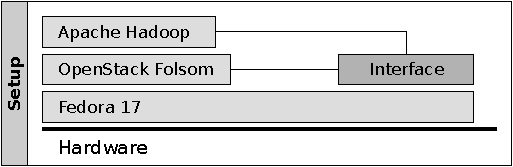
\includegraphics[width=0.45\textwidth]{img/002}
\caption{High level design diagram}
\label{fig:arch1}
\end{figure}



At the right end of Figure \ref{fig:arch1}, it appears an \emph{Interface} module lying on top of Fedora and being connected to both \emph{OpenStack} and \emph{Apache Hadoop}. Its main purpose is to deploy virtual \emph{Hadoop} clusters, to manage its component virtual machines' ---or \emph{VM}s--- lifecycles and to orchestrate \emph{MapReduce} workflows executions.



\subsection{Initial setup}
\noindent \emph{qosh}'s own installation script will automatically configure a highly-performing testing environment that could be easily scaled-out as demand grows. Figure \ref{fig:initial} represents the layered setup decomposition in a single node after the installation procedure had finished.

\begin{figure}[tbp]
\centering
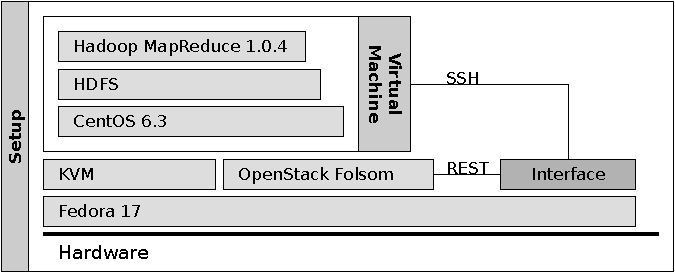
\includegraphics[width=0.45\textwidth]{img/005}
\caption{Layered initial deployment}
\label{fig:initial}
\end{figure}

The \emph{OpenStack} modules deployed are those fundamentally required by a minimum standalone setup:

\begin{description}
 \item[Keystone] manages authorization, authentication and quota by user and \emph{tenant}.
 \item[Nova] handles VMs' lifecycles and networking configuration, routing and data flow utilizing the \emph{Kernel Virtual Machine} (KVM) as hypervisor.
 \item[Glance] holds the browsable catalog of installed VM images on the local file system.
\end{description}

Which implies that no fault tolerance measures are defined ---as expected from a single node and local file system arrangement--- cloud-wise, but it certainly allows for other standard safety protocols to be implemented ---on the order of some RAID level with replication or UPS solutions.


\subsection{Interface}
\noindent Figure \ref{fig:interface} represents the user interface's modular composition. There are three essential modules within:

\begin{figure}[tbp]
\centering
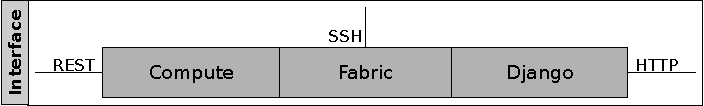
\includegraphics[width=0.45\textwidth]{img/003}
\caption{Interface composition}
\label{fig:interface}
\end{figure}


\subsubsection{Compute}
\noindent \emph{Compute} is the REST access client that bridges the \emph{OpenStack} cloud with the web interface, effectively decoupling \emph{qosh} from the infrastructure provider. It basically encapsulates a series of methods by which an authorized user is allowed to manually define VM deployment behavior.

Current implementation manages virtual clusters defined with \emph{OpenStack} running on a single real cluster, i. e. no hybrid clouds are supported. However, \emph{Compute} may be effortlessly adapted to handle VMs running on other IaaS deployments or to manage hybrid clouds, with no interaction whatsoever with another module, as far as \emph{qosh} API semantics are preserved.


\subsubsection{Fabric}
\noindent \emph{Fabric} is a \emph{Python} library used to simplify managing our virtual cluster by establishing SSH tunnels with the VMs, letting \emph{qosh} shape \emph{Hadoop} configuration, put processing data into HDFS ---Hadoop Distributed File System--- and recover results to user space; everything as SSH traffic.

To establish SSH connections our \emph{Fabric} module is fed a \emph{Keystone}-generated keypair. This keypair is created on each virtual cluster deployment and shared by all VMs in the same cluster. Its private part is injected into VMs once they have finished booting (refer to section \ref{subsec:initsh} for an implementation), and its public part is kept on the local file system. It is automatically removed ---both from \emph{OpenStack} and file system--- when \emph{Apache Hadoop} execution completes.


\subsubsection{Django}
\noindent \emph{Django} glues together both modules, renders HTML to be displayed to the user and organizes result and metadata storage.

\emph{Django} can be plugged different back-ends to deal with varied needs. ------------------------------------------------------------

Putting it all together, a user would define \emph{MapReduce} computations though a Django-backed web interface. Django would pass configuration parameters on to \emph{Fabric} for creating and feeding input data to a virtual \emph{Hadoop} cluster. And lastly, real infrastructure would be provisioned by an IaaS cloud driven through \emph{Compute} module.


\subsection{Deployment}
\noindent \emph{qosh}'s installation script will take care of a single node deployment in an automatic fashion, so no previous knowledge of \emph{OpenStack} or \emph{Hadoop} would be required to exploit \emph{qosh}'s elastic \emph{MapReduce} prowess in this case; though the virtual cluster's \emph{elasticity} would be heavily constrained. To overcome this limitation, \emph{qosh} has been architected to abstract the infrastructure underneath, allowing for any IaaS framework to be deployed at any size ---some \emph{Compute} module's parts would require rewriting, nonetheless, if \emph{OpenStack} were not used.

An installation may be grown from a starting single node setup just by laying out a real IaaS cloud cluster of any size. In fact, any public cloud \emph{Amazon Elastic Compute Cloud}-compatible (EC2-compatible) could be used to expose infrastructure that \emph{qosh} would utilize to spawn virtual clusters of any size.


\section{Apache Hadoop Virtual Machine}\label{sec:hadvm}
\noindent The \emph{Apache Hadoop} installation has been manually configured from scratch inside a virtual machine. What follows is the procedure carried out to yield the VM image.

\begin{itemize}
 \item After a clean Fedora 17 installation, \texttt{yum} was employed to add the \emph{Virtual Machine Manager} (\texttt{virt-manager}) package which would be exerted to sketch the VM. Along with it, \texttt{libvirt}, \texttt{kvm} and \texttt{qemu} were also installed.
 
 \item Using \texttt{virt-manager} a VM was spawned anew with 1 VCPU, 1 GB RAM and 4 GB qcow2 HDD.
 
 \item A \emph{CentOS 6.3} network installation image was booted inside the VM, choosing \emph{Basic Server} as set of packages to be configured within a single \emph{ext4}-formatted partition without LVM.
 
 \item Once completed and self-restarted, the system was updated and \emph{SELinux} relaxed to be \emph{permissive} by issuing:
 
 \begin{verbatim}
[guest]$ sudo yum update -y
[guest]$ sudo setenforce 0
[guest]$ sudo sed -i \
s_SELINUX=enforcing_SELINUX=permissive_ \
/etc/selinux/config
 \end{verbatim}
 
 \item Both \emph{Oracle JRE 1.7} and \emph{Apache Hadoop 1.0.4} were downloaded ---AMD64 and rpm packages---, installed and configured in the VM.
 
 \item Right afterwards, an \texttt{hduser} was added with \texttt{hadoop} as primary group.

 \item \texttt{sshd} was set to disallow either \texttt{root} user connections or the tuple (user, password) as credentials, to effectively limit SSH tunnels to those authorized with (public, private) keypair collations. By using this approach, only the user spawning a virtual cluster would have access to its instances, provided he or she remained the sole acquaintances with the \emph{OpenStack}-injected private keypair.
 
   \begin{verbatim}
[guest]$ sudo sed -i \
s_^#PermitRootLogin\ yes.*_\
PermitRootLogin\ no_ /etc/ssh/sshd_config
[guest]$ sudo sed -i \
s_^PasswordAuthentication\ yes.*_\
PasswordAuthentication\ no_ \
/etc/ssh/sshd_config
[guest]$ sudo rm -rf /home/hduser/.ssh
[guest]$ sudo rm -f /etc/ssh_host*
   \end{verbatim}
   
 \item Three scripts were written (refer to appendix \ref{sec:apx}) and placed in \texttt{/etc/init.d/} to convey user configuration to the VM and to secure access.
 
 \item With \texttt{yum groups}, unused sets of services and applications ---like \texttt{Xserver}--- were removed from the system in order to trim its size and memory footprint.
 
 \item Subsequently, the qcow2 HDD image was packed in two steps. Initially, the beginning offset of the partition inside the image was trimmed by exposing only that partition with \texttt{qemu-nbd}. Right afterwards, its contents were dumped into a new partitionless image. Then, a long zero-file was generated to fill up all the remaining free space in the image, so that \texttt{qemu-img} be adequately executed to do the real compressing. Once \texttt{qemu-img} had completed processing, the image file in the host system was neatly compressed but the image's file system reported no free space, clogged up with the zero-file that had to be manually removed.
 
   \begin{verbatim}
[host]$ sudo modprobe nbd max_part=8
[host]$ sudo qemu-nbd -c /dev/nbd0 \
-P 1 original.qcow2
[host]$ dd if=/dev/nbd0 of=trimmed.qcow2
[host]$ sudo qemu-nbd -d /dev/nbd0

[host]$ sudo qemu-nbd -c /dev/nbd0 \
trimmed.qcow2
[host]$ sudo mkdir /mnt/img
[host]$ sudo mount /dev/nbd0 /mnt/img
[host]$ sudo dd if=/dev/zero \
of=/mnt/img/root/zeros bs=1M count=4K
[host]$ sudo umount /mnt/img
[host]$ sudo qemu-nbd -d /dev/nbd0
[host]$ qemu-img convert -c -p -f qcow2 \
-O qcow2 trimmed.qcow2 compacted.qcow2

[host]$ sudo qemu-nbd -c /dev/nbd0 \
compacted.qcow2
[host]$ sudo mount /dev/nbd0 /mnt/img
[host]$ sudo rm -f /mnt/img/root/zeros
   \end{verbatim}
   
 \item Lastly, both \emph{initram} and \emph{kernel} were copied out to the host machine and \texttt{nbd0} disconnected.
 
 \begin{verbatim}
[host]$ sudo cp /mnt/img/boot/initramfs-\
$(uname -r).img
/mnt/img/boot/vmlinuz-$(uname -r)
[host]$ sudo umount /mnt/img
[host]$ sudo qemu-nbd -d /dev/nbd0
 \end{verbatim}

\end{itemize}







\section{Execution}\label{sec:execution}
\noindent

\begin{figure*}[tbp]
\centering
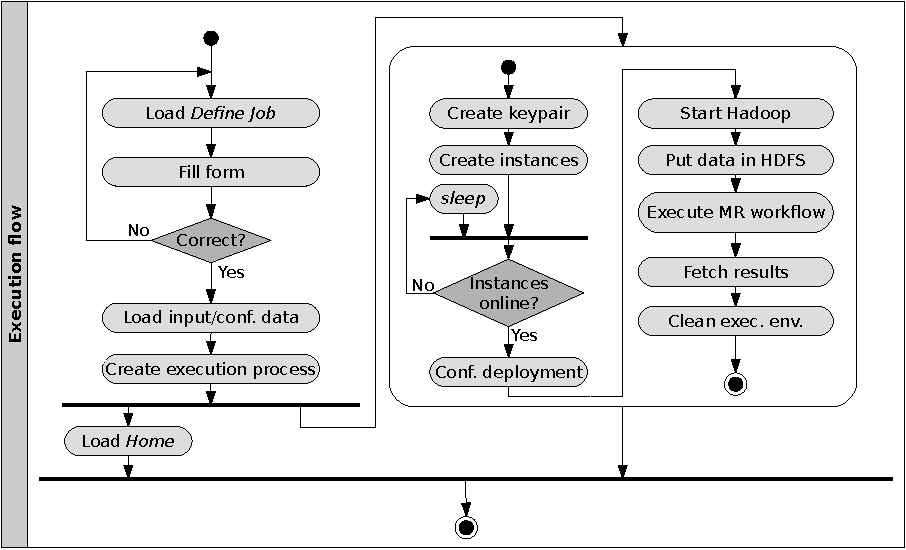
\includegraphics[width=0.65\textwidth]{img/006}
\caption{Global execution flow}
\label{fig:exflow}
\end{figure*}


\section{Performance}\label{sec:performance}


\bibliographystyle{abbrv}
\bibliography{qosh-paper}

\appendix

\section{Cloud-init scripts}\label{sec:apx}
\subsection{cloud-prenet.sh}

\begin{verbatim}
#!/bin/sh
#
# Custom script to control pre-network
# initialization
#
# Remove ssh Keys DSA, RSA & HOST
rm -f /etc/ssh/*host*

# Remove persistent-net-rules
rm -f /etc/udev/rules.d/70-persistent-net.rules

# Remove history
rm -f /home/hduser/.bash_history\
 /root/.bash_history
\end{verbatim}


\subsection{cloud-init.sh}\label{subsec:initsh}

\begin{verbatim}
#!/bin/sh
#
# Simple cloud-init script to fetch
# meta-data injected into instances
# in order to configure them

fetch_and_set() {

  response_code="$(\
   curl -sI http://169.254.169.254/1.0/\
   meta-data/hostname | grep HTTP\
   | awk {'print $2'})"
  
  if [ "$response_code" == "200" ]
  then
    new_hostname="$(\
     curl -s http://169.254.169.254/1.0/\
     meta-data/hostname)"
    sed -i 's/'"$HOSTNAME"'/'"$new_hostname"\
     '/g' /etc/hosts /etc/sysconfig/network
    HOSTNAME=$new_hostname
    hostname $new_hostname
  fi
  
  response_code="$(\
   curl -sI http://169.254.169.254/1.0/\
   meta-data/public-keys/0/openssh-key\
   | grep HTTP | awk {'print $2'})"

  if [ "$response_code" == "200" ]
  then
    rm -rf /home/hduser/.ssh
    mkdir -p /home/hduser/.ssh

    curl -s http://169.254.169.254/1.0/\
     meta-data/public-keys/0/openssh-key\
     | grep 'ssh-rsa' >> \
     /home/hduser/.ssh/authorized_keys
    
    chown -R hduser:hadoop /home/hduser/.ssh
    echo -e "\nAUTHORIZED_KEYS:"
    echo "************************"
    cat /home/hduser/.ssh/authorized_keys
    echo "************************"
  fi

}

# Change hostname to match meta-data
# instance name if found
#
http_response_code="$(\
 curl -sI http://169.254.169.254/1.0/\
 | grep HTTP | awk {'print $2'})"

[ "$http_response_code" != "200" ] && \
echo -e "\nWARNING: No meta-data found!\n"\
 && exit 1

fetch_and_set
\end{verbatim}


\subsection{cloud-shtdwn.sh}

\begin{verbatim}
#!/bin/sh
#
# Remove ssh Keys DSA, RSA & HOST
rm -f /etc/ssh/*host*

# Remove ssh authorized_keys
rm -f /root/.ssh/authorized_keys\
 /home/hduser/.ssh/authorized_keys

# Remove persistent-net-rules
rm -f /etc/udev/rules.d/\
70-persistent-net.rules

# Remove history
rm -f /home/hduser/.bash_history\
 /root/.bash_history

# Remove hadoop logs
rm -rf /var/log/hadoop/hduser

# Clear some system logs
for file in $(ls -F /var/log |grep -ve "/$")
do
  echo > /var/log/$file
done
\end{verbatim}


\end{document}
